\chapter{ANGULAR SENSING AND CONTROL CALIBRATIONS}
\label{ch:ASCcal}
The typical method of calibrating a digital channel is to inject a
signal of known amplitude into the system and take the ratio with the
amplitude of the digital measurement of the signal.
% Two ways of
% determining the physical amplitude of the injected signal are
% \textcolor{blue}{(see if I can classify calibration methods)}
% \begin{itemize}
% \item 
% \item 
% \end{itemize}
I describe in this appendix the calibrations I made of some of the
angular sensing channels.
%, all the while demonstrating particular examples of these methods.

% \section{Calibrations}
% Because the data is collected digitally, the units are in digital
% counts. This must be converted into physical units in order to
% facilitate comparison to models and to make meaningful statements. The
% typical method of calibrating a digital channel is to inject a signal
% of known amplitude into the system and take the ratio with the
% amplitude of the digital measurement of the signal. Two ways of
% determining the physical amplitude of the injected signal are
% \textcolor{blue}{(see if I can classify calibration methods)}
% \begin{itemize}
% \item 
% \item 
% \end{itemize}
% I describe in this section the calibrations I made of some of the
% angular sensing channels, all the while demonstrating particular
% examples of these methods.


\section{Beam Spot Motion}
\label{sec:bsmcal}
A quantity of interest is how much the beam moves on the ITMs and
ETMs. It is this beam spot motion which, together with the mirror
angular motion, creates a length signal that contributes noise to
DARM. An elegant way of following the motion of the beam on the test
masses is to track pickoffs of the light transmitted or reflected from
the mirrors. We have such signals naturally available for the ETMs and
ITMs from the QPDs which are otherwise used for ASC sensing. For
example, QPDX and QPDY see the light transmitted through each of the
ETMs and WFS2 sees the pickoff of light from the wedge of ITMX.

To calibrate the counts of the QPD and WFS2 pitch and yaw error
signals,\footnote{\texttt{L1:ASC-QPDY\_\{PIT,YAW\}\_IN1} and
\texttt{L1:ASC-WFS2\_DC\{Pitch, Yaw\}Mon}} I moved the beam a
known distance on the test mass, $\Delta x$, and recorded the
corresponding $\Delta y$ of the QPD and WFS2 readback. The ratio
$\Delta x /\Delta y$ is the calibration from counts to meters. The
details of the procedure are described below.


\subsection{Moving the Beam} 
Moving the beam on the mirrors in a controlled fashion is
straightforward because of the ASC system. All that we need to do is
introduce an offset to the setpoint of the of the beam centering
aspect of the ASC servo. For the ETMs we put a DC offset in the
\texttt{L1:ASC-QPD\{X,Y\}\_\{PIT, YAW\}\_\{OFFSET\}} channel and for
the ITMs we changed the $X$ and $Y$ targets of the beam splitter beam
centering servo.

\subsection{Measuring How Much the Beam Has Moved} 
The more difficult task is measuring just how much the beam has
moved. For this, we make use of the lever arm mechanism of angle to
length coupling as explained in Section~\ref{sec:tolerance}. The
concept of the measurement is to move the axis of rotation of the
mirror so that it passes through the center of the beam. We use the
OSEMs to change the location of the axis of rotation, and we use DARM
to determine when the axis is aligned with the beam center. For
example, if we drive the top two OSEMs more than the bottom two OSEMs,
we've created an axis of rotation that sits below the center of
mass. The result of such tuning is an effective rebalance of the
center of mass of the mirror so that it is aligned with the center of
the beam. The procedure is:
\begin{itemize}
\item Shake the mirror at some frequency $f$ (we use
39.5 Hz) during a full lock \vspace{-10pt}
\item Demodulate DARM at $f$ for several different sets of OSEM gains \vspace{-10pt}
\item Fit a quadratic to the demodulated data to pinpoint the OSEM gains that
  minimize the coupling to DARM
\end{itemize}

\begin{figure}
\begin{centering}
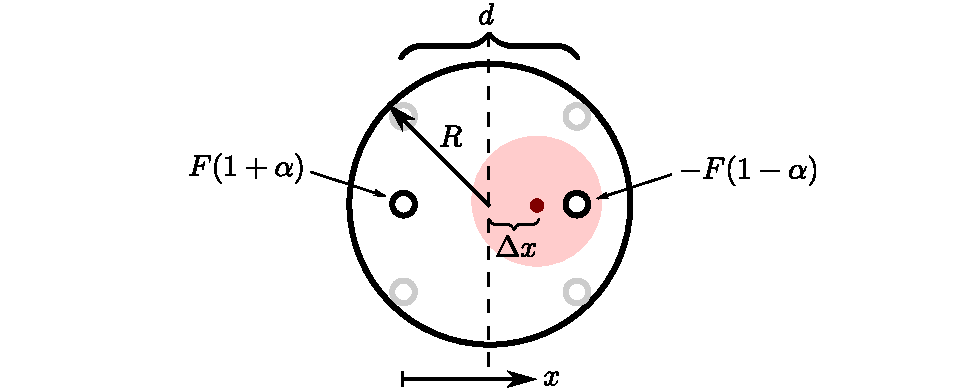
\includegraphics{figures/geometry_mirror_osems.pdf}
\caption[Diagram of mirror and OSEM geometry]{Geometry of OSEMs and
  mirror as used for calculating the location of the axis of rotation
  when the torques are unequal.}
\label{fig:mirror_osem_geometry}
\end{centering}
\end{figure}

Relating the OSEM gains to absolute beam position on the mirror
requires only the geometry of the mirror and OSEM setup as sketched in
Figure \ref{fig:mirror_osem_geometry}. We estimate the OSEM locations as
being on the edge of the mirror such that the length $d$ of one side
of the square that they form is given by $d =\sqrt{2} R$, where $R =
12.5$ cm is the radius of the mirror. Then, collapsing the four OSEMs
into a representative two at the centers of two opposite sides of the
square and assigning them gains of $1 + \alpha$ and $-(1-\alpha)$ for
a force $F$, we can evaluate where the pivot point $x$ is located by
setting the sum of the torques equal to zero:
\begin{equation}
F [1+\alpha] x = F [1-\alpha][d-x].
\end{equation}
Therefore, the beam location relative to center, $\Delta x$, is
\begin{equation}
\Delta x := \frac{d}{2} - x = \alpha \frac{d}{2},
\end{equation}
and for a change in a pitch or yaw coil gain, the change in beam
position, $\Delta x$, is:
\begin{equation}
|\Delta{x}| = \frac{|\Delta{\mbox{gain}}| R}{\sqrt{2}} .
\end{equation}
The final calibrations of these channels are shown in Table
\ref{table:bsmcal}. \footnote{A minor technicality is that since there
  are no filters between the QPD error signals and the offset channel,
  their units are exactly the same. Thus, calculating meters of beam
  spot motion as a function of offset serves to calibrate the error
  point. For convenience, this is what I did.}

\begin{table}
\centering
\caption[Beam spot motion calibrations]{Calibrations to be used with
 the QPDX, QPDY, and WFS2 DC pitch and yaw error signals for a
 measure of beam spot motion.} 
\begin{tabular}{l l l l}
\hline
         & ETMX & ETMY & ITMs \\
\hline
pitch & $1.03\times10^{-5}$ m/ct & $1.21\times10^{-5}$ m/ct & $5.52\times10^{-2}$ m/ct \\
yaw & $0.88\times10^{-5}$ m/ct & $0.80\times10^{-5}$ m/ct & $4.79\times10^{-2}$ m/ct \\
\hline
\end{tabular}
\label{table:bsmcal}
\end{table}



\section{Angular Mirror Motion}
\label{sec:oplevcal}
The optical levers provide a straightfoward measure of individual
mirror motion. The channels I calibrated were of the form
\texttt{L1:SUS-ETMX\_OPLEV\_\{P,Y\}ERROR}, the optical lever error
signals for each of the large optics. I made use of the dependence of
power in a misaligned cavity (refer to Appendix~\ref{sec:cavitypower})
to calibrate the ETM and ITM optical levers, and used a less precise,
rudimentary method to calibrate the RM, BS, and MMT3 optical levers.

\subsection{ETM and ITM Optical Levers} 
I calibrated the arm cavity optical levers by tracking the power loss
in the locked arm as one of its mirrors is tilted. The closed form
expression for cavity power as a function of mirror tilt is derived in
Appendix \ref{sec:cavitypower}. All that is needed is a quadratic fit
to the data collected. From the fit parameters, I can determine the
factor, $\Delta \theta / \Delta y$, which converts the digital counts
of the optical lever channel, $y$, to units of radians.

To make the measurement, I locked a single arm and maximized the power
build up. Then I slowly stepped the pitch or yaw pointing of one of
the mirrors away to one side of resonance, and then back and to the
other side, repeating this several times. All the while, I recorded
the optical lever error signal of the mirror whose angle I was
changing, and the power in the arm as determined from the amount of
light transmitted through the
ETMs.\footnote{\texttt{L1:LSC-NPTR\{X,Y\}\_OUT16}}

From Eq.~\ref{eq:pwr_disptilt}, we see that the power in the arm, $P$,
is a function of the form 
\begin{equation}
P = P_{max} \exp{[-b (y-y_0)^2]},
\label{eq:OLcalfit}
\end{equation}
where $y_0$ is the DC offset of the optical lever channel and $b$ is
related to physical cavity axis displacement $a$ and tilt $\alpha$ by
$by^2~=~(a/w_0)^2+(\alpha/\theta_0)^2$. In order to relate the optical
lever signal, $y$, to physical cavity parameters, we divide by
$\Delta{\theta}^2$ and rearrange to get:
\begin{equation}
\frac{\Delta \theta}{\Delta y} = \sqrt{b} \left[
  \left[\frac{\Delta a/\Delta\theta}{w_0}\right]^2 +
  \left[\frac{\Delta\alpha/\Delta\theta}{\theta_0}\right]^2
\right]^{-\frac{1}{2}} .
\end{equation}
The terms in the numerators on the right hand side are fixed constants
based on the cavity geometry and can be calculated using
Eq. \ref{eq:cavitydisptilt_mirrorangle}. The measurement data and fits
are shown for both pitch and yaw in Figure \ref{fig:OLcal}. The ETM
optical levers make use of a broader range of optical lever signal
than do the ITMs. (Also note that the maximum power in the y-arm is about
10\% less than that in the x-arm. This is true at both Hanford and
Livingston, and is due to the priority given to the x-arm in the
alignment scheme, as explained in Appendix
\ref{sec:initial_alignment}.)

\begin{figure}
\begin{centering}
\subfigure{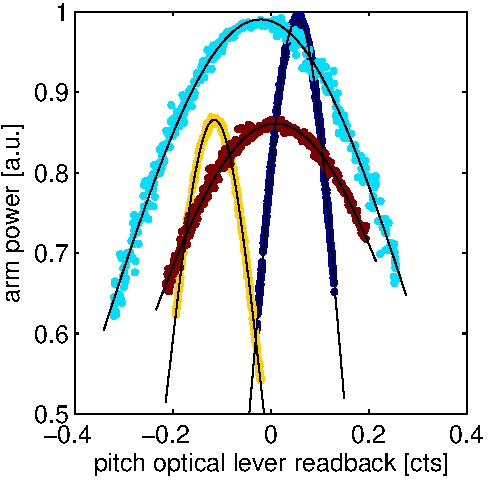
\includegraphics[width=0.5\columnwidth]{figures/olcal_pitch.pdf}}\subfigure{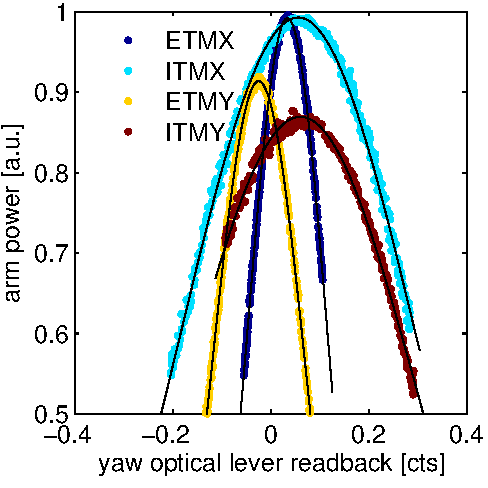
\includegraphics[width=0.5\columnwidth]{figures/olcal_yaw.pdf}}
%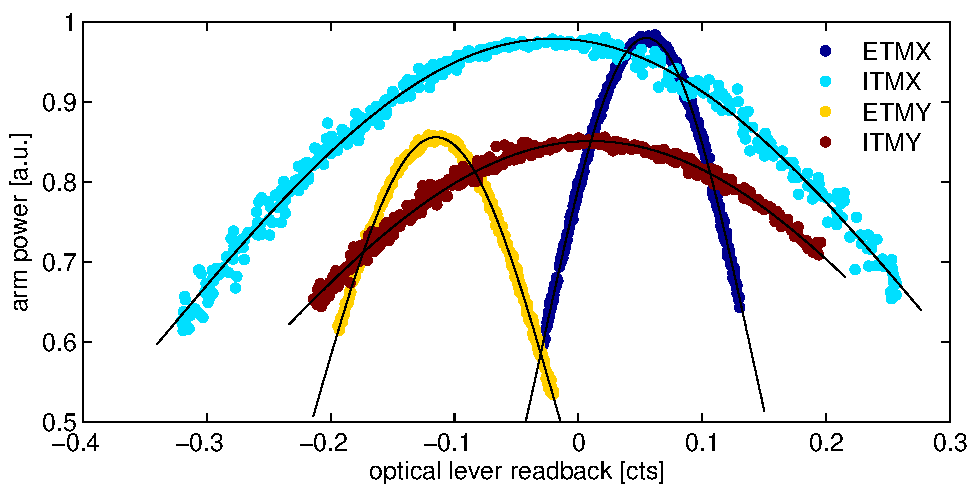
\includegraphics[width=1.0\columnwidth]{figures/oplevcal_pitch.pdf}
\caption[Optical lever calibration data.]{Optical lever calibration data and
  fits to Eq. \ref{eq:OLcalfit}.}
\label{fig:OLcal}
\end{centering}
\end{figure}


\subsection{RM, BS, and MMT3 Optical Levers}
To calibrate the RM, BS and MMT3 optical levers, I used my own eyes
and the camera images and known dimensions of the ETM beam cages. With
the interferometer unlocked, I moved the optics in pitch and yaw,
tracking the beam's movement on the ETM cages. In order to calibrate
the RM, I used the reflection off ITMY to the RM and onto the ETMY
cage. The BS and MMT3 required only straight shots to the ETMs. For
yaw, I moved the mirrors until the beam was centered on each vertical
suspension post, and for pitch I moved the beam from the center of the
mirror to the top of the cage. The beam moves by $x = 2\theta$ on
across the cage when the mirror moves by $\theta$, so with small angle
approximations, the mirror angle is simply $x/2L$ where $L$ is the
distance from mirror to ETM cage.

The final $\Delta\theta / \Delta x$ calibrations of all optical levers
are in Table \ref{table:oplevcal}. 

\begin{table}
\centering
\caption[Optical lever calibrations]{Calibrations to be used
  with the optical lever error signals 
  for a measure of angular mirror motion. Units are \microrad/ct.}
\begin{tabular}{l l l l l l l l}
\hline
        & ETMX & ETMY & ITMX & ITMY & RM & BS & MMT3 \\
\hline
pitch & 49.4 & 43.0 & 14.9 & 15.6 & 61.9 & 47.3 & 57.4 \\
yaw & 50.7 & 43.3 & 20.1 & 20.2 & 42.5 & 63.5 & 55.5 \\
\hline
\end{tabular}
\label{table:oplevcal}
\end{table}



\section{WFS Error Signals}
\label{sec:cal_sensing}
The WFS error signals\footnote{i.e. \texttt{L1:ASC-WFS1\_QP}} are physically
Watts of power at the detectors, which the WFS electronics convert
into a voltage. To turn WFS counts into voltage of signal at the
output of the detector, we must backtrack through the electronics and
calibrate the WFS demodulation chain.

% The WFS error signals (i.e. \texttt{L1:ASC-WFS1\_Q1}) are physically
% Watts of power at the detectors. Converting the error signal in
% digital counts to Watts requires working backwards through the
% electronics, and can be divided into two parts. First, we must
% calibrate the WFS demodulation chain to backtrack WFS counts into
% voltage of signal at the input to the mixer. Second, we must convert
% voltage at the mixer into Watts at the sensor based on properties of
% the photodetector RF electronics. \textcolor{blue}{For now, it
%   suffices to calibrate the signal in Volts.}

%\subsubsection{Counts to Volts} 
The analog to digital RF chain for the WFS includes a demodulation
board, a whitening board, an anti-alias board, and the ADC. I
calibrated this chain by injecting a sine wave of the same frequency
as a typical WFS signal, yet of known voltage into the WFS
demodulation board. Comparing the peak to peak voltage of this input
sine wave to the peak to peak amplitude of the resulting digital
counts signal provides the Volts per count conversion. The
calibrations are presented in Table \ref{table:demodcal}.

\begin{table}
\centering
\caption[Demodulation chain calibration for each quadrant of each
 WFS]{Demodulation chain calibration for each quadrant of each
 WFS. Units are \micro V/count.}
\begin{tabular}{l l l l l l}
\hline
 & q1 & q2 & q3 & q4 & average \\
\hline
 WFS1  & 0.35 &   0.32 &   0.34 &   0.35 & 0.34 \\
 WFS2  & 8.8 &   8.6 &   8.7  &  8.5 & 8.7       \\
 WFS3  & 6.4 &   5.8 &   5.8 &   5.7 & 5.9     \\
 WFS4  & 6.3 &   5.4 &   5.3  &  7.4 & 6.1    \\
\hline
\end{tabular}
\label{table:demodcal}
\end{table}

It should be noted that the demodulation chain calibration numbers for
all quadrants of a particular WFS differ no more than 20\% from the
average. The demodulation chain does not significantly distort the
error signals.


% \subsubsection{Volts to Watts}
% The voltage created per Watt of signal on the WFS is determined by the
% responsivity (Amps/Watt) and transimpedance (Volts/Amp) of the
% diode. A model of the 25~MHz WFS transimpedance is shown in
% Figure \ref{fig:wfs25MHzTF}, indicating a magnitude of 90~dB at
% 25~MHz. The responsivity is found in Section \ref{sec:pds}. It is
% 0.86~A/W. 

% The final WFS calibration numbers are found in Table \ref{tab:WFScal}.

% \begin{figure}
% \begin{centering}
% 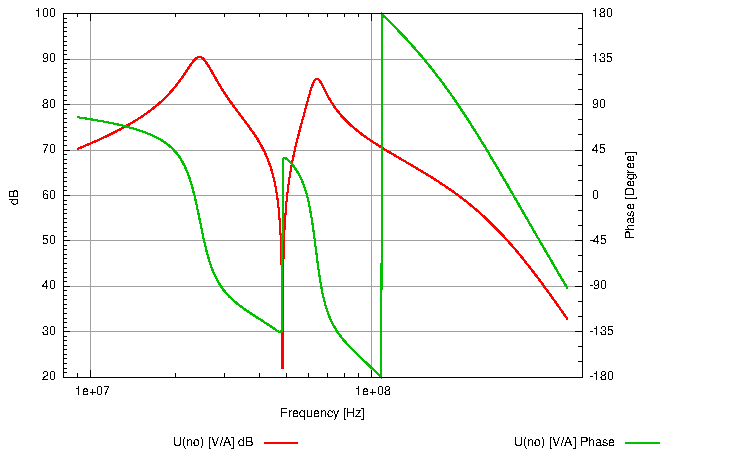
\includegraphics[width=1.0\textwidth]{figures/wfs25MHzTF.pdf}
% \caption{Transimpedance of the 25 MHz resonant RF WFS front end
%   electronics. The model was made using software called LISO.}
% \label{fig:wfs25MHzTF}
% \end{centering}
% \end{figure}

% \begin{table}
% \centering
% \caption[]{WFS error signal calibrations from digital counts to Watts.}
% \begin{tabular}{l l l l}
% \hline
% WFS1 & WFS2 & WFS3 & WFS4 \\
% \hline
% $3.9\times10^{-16}$ & $1.0\times10^{-14}$ & & \\
% \hline
% \end{tabular}
% \label{table:WFScal}
% \end{table}



\section{Angular Optical Gain}
\label{sec:cal_opticalgain}
The calibrated WFS sensing matrix (using the calibration presented in
Sec.~\ref{sec:cal_sensing}) can be used in conjuction with the
simultaneously measured drive matrix (as described in
Sec.~\ref{sec:mirrorgains}) to calculate the angular optical
gain. Each row of the sensing matrix must be divided by the measured
amplitude of that row's DOF excitation, which is found as the diagonal
elements of Table~\ref{table:excitations_calibrated}. The result of
doing so gives the angular optical gain of the interferometer in terms
of WFS Volts per radian.
